\documentclass[tikz, border=12pt]{standalone}
\usepackage{tikz}
\usepackage{amsmath, amssymb}
\usetikzlibrary{arrows.meta, positioning, calc, backgrounds}

% Colors consistent with model_figure.tex
\definecolor{cBlue}{RGB}{159,197,232}
\definecolor{cGray}{RGB}{215,215,215}
\definecolor{cYellow}{RGB}{255,229,153}
\definecolor{cOrange}{RGB}{255,193,120}
\definecolor{cGreen}{RGB}{167,210,167}
\definecolor{cTeal}{RGB}{86,180,170}
\definecolor{cPurple}{RGB}{196,175,222}
\definecolor{cRed}{RGB}{200,60,60}

\begin{document}
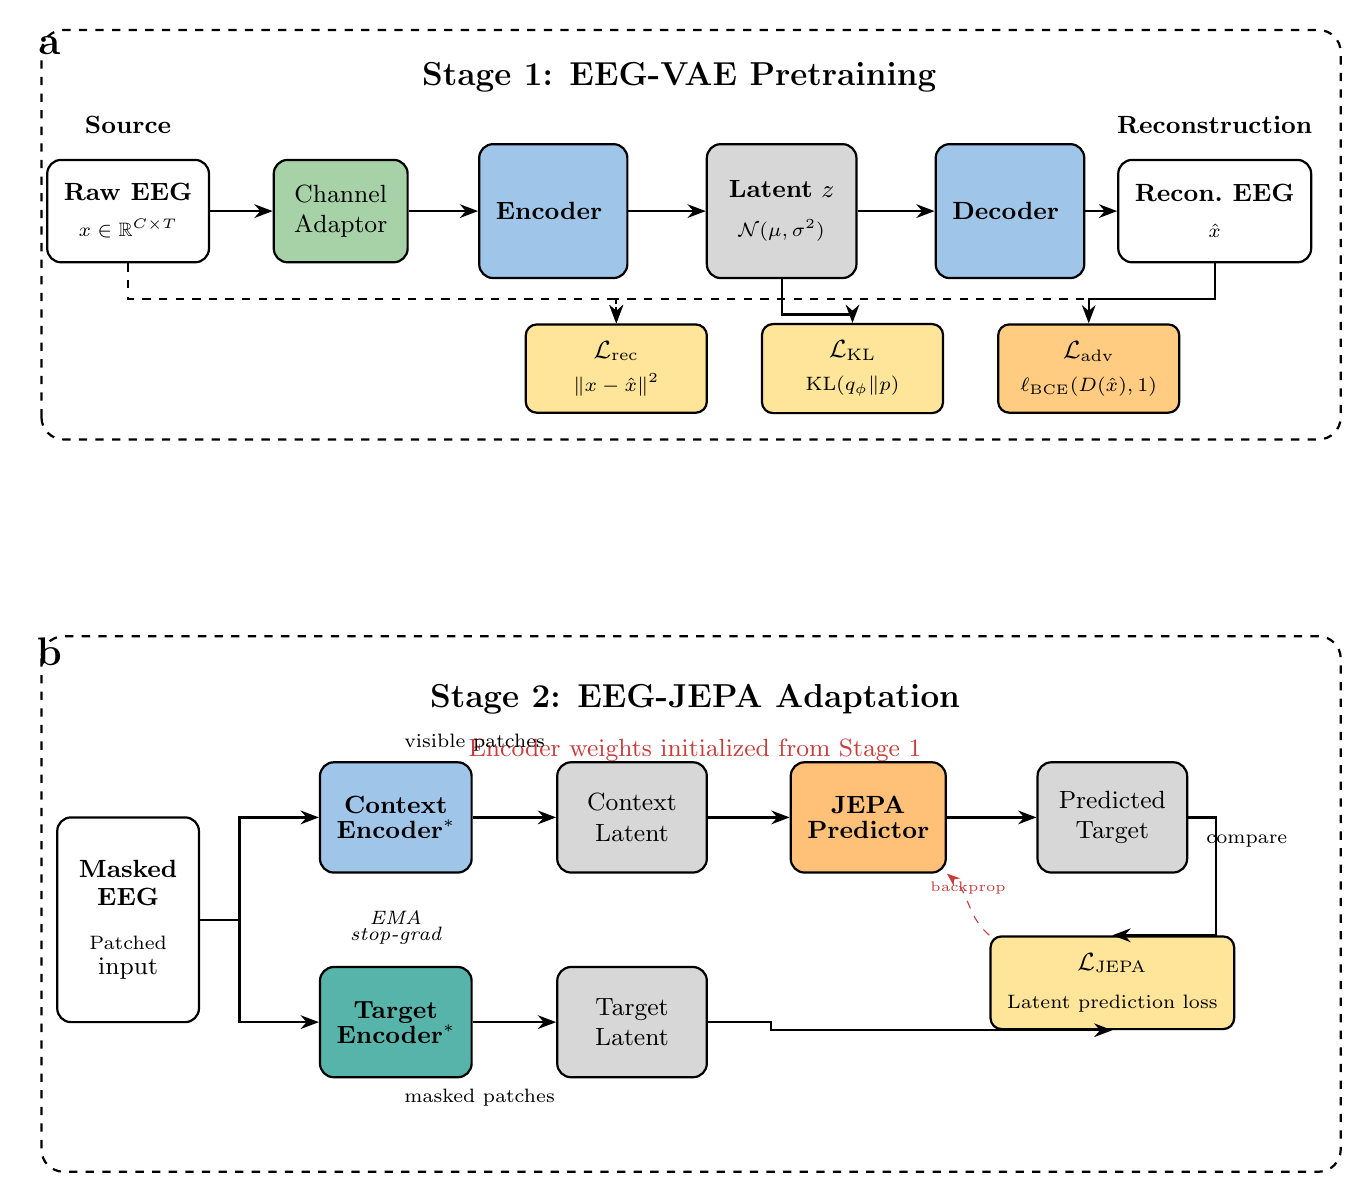
\begin{tikzpicture}[
  >=Stealth, thick,
  block/.style={draw, rounded corners=5pt, align=center, inner sep=6pt, font=\small},
  loss/.style={draw, rounded corners=4pt, align=center, fill=cYellow,
               inner sep=6pt, font=\small},
  arr/.style={->, thick, >=Stealth},
  darr/.style={->, dashed, thick, >=Stealth}
]

%%=============================================================================
%% PANEL A — Stage 1: EEG-VAE Pretraining
%%=============================================================================

%% Source / Reconstruction labels
\node[font=\small\bfseries] at (1.0, 5.1) {Source};
\node[font=\small\bfseries] at (14.8, 5.1) {Reconstruction};

%% Main flow
\node[block, fill=white, minimum width=1.7cm, minimum height=1.3cm]
  (raw_a) at (1.0, 4.0) {
  \textbf{Raw EEG}\\[2pt]\scriptsize $x \in \mathbb{R}^{C \times T}$
};
\node[block, fill=cGreen, minimum width=1.7cm, minimum height=1.3cm]
  (adapt_a) at (3.7, 4.0) {
  Channel\\Adaptor
};
\node[block, fill=cBlue, minimum width=1.7cm, minimum height=1.7cm]
  (enc_a) at (6.4, 4.0) {
  \textbf{Encoder}
};
\node[block, fill=cGray, minimum width=1.9cm, minimum height=1.7cm]
  (lat_a) at (9.3, 4.0) {
  \textbf{Latent} $z$\\[3pt]\scriptsize $\mathcal{N}(\mu,\sigma^2)$
};
\node[block, fill=cBlue, minimum width=1.7cm, minimum height=1.7cm]
  (dec_a) at (12.2, 4.0) {
  \textbf{Decoder}
};
\node[block, fill=white, minimum width=1.7cm, minimum height=1.3cm]
  (recon_a) at (14.8, 4.0) {
  \textbf{Recon.\ EEG}\\[2pt]\scriptsize $\hat{x}$
};

%% Loss boxes
\node[loss, minimum width=2.3cm] (l_rec_a) at (7.2, 2.0) {
  $\mathcal{L}_{\mathrm{rec}}$\\[1pt]\scriptsize $\|x - \hat{x}\|^2$
};
\node[loss, minimum width=2.3cm] (l_kl_a) at (10.2, 2.0) {
  $\mathcal{L}_{\mathrm{KL}}$\\[1pt]\scriptsize $\mathrm{KL}(q_\phi \| p)$
};
\node[loss, fill=cOrange!70!cYellow, minimum width=2.3cm] (l_adv_a) at (13.2, 2.0) {
  $\mathcal{L}_{\mathrm{adv}}$\\[1pt]\scriptsize $\ell_{\mathrm{BCE}}(D(\hat{x}),1)$
};

%% Title
\node[font=\large\bfseries] at (8.0, 5.7) {Stage 1: EEG-VAE Pretraining};

%% Main flow arrows
\draw[arr] (raw_a)   -- (adapt_a);
\draw[arr] (adapt_a) -- (enc_a);
\draw[arr] (enc_a)   -- (lat_a);
\draw[arr] (lat_a)   -- (dec_a);
\draw[arr] (dec_a)   -- (recon_a);

%% Loss arrows
% Both raw and recon feed L_rec (dashed = comparison, not gradient path)
\draw[darr] (raw_a.south)   -- ++(0,-.45) -| (l_rec_a.north);
\draw[darr] (recon_a.south) -- ++(0,-.45) -| (l_rec_a.north);
% KL from latent
\draw[arr]  (lat_a.south)   -- ++(0,-.45) -| (l_kl_a.north);
% Adv from recon
\draw[arr]  (recon_a.south) -- ++(0,-.45) -| (l_adv_a.north);

%% Panel A dashed border + label
\draw[dashed, thick, rounded corners=8pt]
  (-0.1, 1.1) rectangle (16.4, 6.3);
\node[font=\Large\bfseries] at (-0.0, 6.1) {\textbf{a}};

%%=============================================================================
%% PANEL B — Stage 2: EEG-JEPA Adaptation
%%=============================================================================

%% Masked EEG input (vertically centered between the two paths)
\node[block, fill=white, minimum width=1.8cm, minimum height=2.6cm]
  (masked) at (1.0, -5.0) {
  \textbf{Masked}\\[-1pt]\textbf{EEG}\\[5pt]
  \scriptsize Patched\\[-2pt]input
};

%% TOP PATH — visible patches
\node[block, fill=cBlue, minimum width=1.9cm, minimum height=1.4cm]
  (ctx_enc) at (4.4, -3.7) {
  \textbf{Context}\\[-2pt]\textbf{Encoder}$^*$
};
\node[block, fill=cGray, minimum width=1.9cm, minimum height=1.4cm]
  (ctx_lat) at (7.4, -3.7) {
  Context\\Latent
};
\node[block, fill=cOrange, minimum width=1.9cm, minimum height=1.4cm]
  (jepa_pred) at (10.4, -3.7) {
  \textbf{JEPA}\\[-2pt]\textbf{Predictor}
};
\node[block, fill=cGray, minimum width=1.9cm, minimum height=1.4cm]
  (pred_tgt) at (13.5, -3.7) {
  Predicted\\Target
};

%% BOTTOM PATH — target patches (EMA encoder)
\node[block, fill=cTeal, minimum width=1.9cm, minimum height=1.4cm]
  (tgt_enc) at (4.4, -6.3) {
  \textbf{Target}\\[-2pt]\textbf{Encoder}$^*$
};
\node[block, fill=cGray, minimum width=1.9cm, minimum height=1.4cm]
  (tgt_lat) at (7.4, -6.3) {
  Target\\Latent
};

%% JEPA loss box
\node[loss, minimum width=2.6cm] (l_jepa) at (13.5, -5.8) {
  $\mathcal{L}_{\mathrm{JEPA}}$\\[3pt]
  \scriptsize Latent prediction loss
};

%% Titles
\node[font=\large\bfseries] at (8.2, -2.2) {Stage 2: EEG-JEPA Adaptation};
\node[font=\small, text=cRed] at (8.2, -2.85)
  {Encoder weights initialized from Stage 1};

%% Path annotations
\node[font=\scriptsize, above right=0.0cm and -1.0cm of ctx_enc]
  {visible patches};
\node[font=\scriptsize, below right=0.0cm and -1.0cm of tgt_enc]
  {masked patches};
% EMA label between the two encoder columns
\node[font=\scriptsize\itshape, align=center]
  at ($(ctx_enc)!0.5!(tgt_enc) + (0, -0.1)$) {EMA\\[-2pt]stop-grad};

%% compare label
\node[font=\scriptsize, right=0.1cm of pred_tgt, yshift=-0.3cm]
  {compare};

%% Arrows — top path
\draw[arr] (masked.east) -- ++(0.5,0) |- (ctx_enc.west);
\draw[arr] (ctx_enc)     -- (ctx_lat);
\draw[arr] (ctx_lat)     -- (jepa_pred);
\draw[arr] (jepa_pred)   -- (pred_tgt);

%% Arrows — bottom path
\draw[arr] (masked.east) -- ++(0.5,0) |- (tgt_enc.west);
\draw[arr] (tgt_enc)     -- (tgt_lat);

%% Arrows — into loss
\draw[arr] (pred_tgt.east) -- ++(0.35,0) |- (l_jepa.north);
\draw[arr] (tgt_lat.east)  -- ++(0.8, 0) |- (l_jepa.south);

%% Backprop arrow (dashed, from loss back to predictor)
\draw[darr, color=cRed, thin]
  (l_jepa.north west) to[out=140, in=-40]
  node[midway, above, font=\tiny, text=cRed] {backprop}
  (jepa_pred.south east);

%% Panel B dashed border + label
\draw[dashed, thick, rounded corners=8pt]
  (-0.1, -1.4) rectangle (16.4, -8.2);
\node[font=\Large\bfseries] at (-0.0, -1.6) {\textbf{b}};

\end{tikzpicture}
\end{document}
